\documentclass[review]{elsarticle}

\usepackage{times}
\usepackage{epsfig}
\usepackage{graphicx}
\usepackage{amsmath}
\usepackage{amssymb}
\usepackage{multirow}
\usepackage{longtable}
\usepackage{color}
\usepackage{rotating}
\usepackage{makecell}
\usepackage{array}
\usepackage{booktabs}
\usepackage{colortbl}
\usepackage{arydshln}
\usepackage{mathrsfs}
\usepackage{amsmath}
\usepackage{lineno,hyperref}
\modulolinenumbers[5]

\journal{Pattern Recognition}

%%%%%%%%%%%%%%%%%%%%%%%
%% Elsevier bibliography styles
%%%%%%%%%%%%%%%%%%%%%%%
%% To change the style, put a % in front of the second line of the current style and
%% remove the % from the second line of the style you would like to use.
%%%%%%%%%%%%%%%%%%%%%%%

%% Numbered
%\bibliographystyle{model1-num-names}

%% Numbered without titles
%\bibliographystyle{model1a-num-names}

%% Harvard
%\bibliographystyle{model2-names.bst}\biboptions{authoryear}

%% Vancouver numbered
%\usepackage{numcompress}\bibliographystyle{model3-num-names}

%% Vancouver name/year
%\usepackage{numcompress}\bibliographystyle{model4-names}\biboptions{authoryear}

%% APA style
%\bibliographystyle{model5-names}\biboptions{authoryear}

%% AMA style
%\usepackage{numcompress}\bibliographystyle{model6-num-names}

%% `Elsevier LaTeX' style
\bibliographystyle{elsarticle-num}
%%%%%%%%%%%%%%%%%%%%%%%

\begin{document}

\begin{frontmatter}

%\title{Elsevier \LaTeX\ template\tnoteref{mytitlenote}}
%\tnotetext[mytitlenote]{Fully documented templates are available in the elsarticle package on \href{http://www.ctan.org/tex-archive/macros/latex/contrib/elsarticle}{CTAN}.}

\title{Covariance Descriptors on a Gaussian Manifold and their Application to Image Set Classification}


%% Group authors per affiliation:
%\author{Elsevier\fnref{myfootnote}}
%\address{Radarweg 29, Amsterdam}
%\fntext[myfootnote]{Since 1880.}


%% or include affiliations in footnotes:
\author[mymainaddress]{Kai-Xuan Chen}
\author[mymainaddress]{Jie-Yi Ren}
%\ead[url]{www.elsevier.com}

\author[mymainaddress]{Xiao-Jun Wu\corref{mycorrespondingauthor}}
\cortext[mycorrespondingauthor]{Corresponding author}
\ead{wu\_xiaojun@jiangnan.edu.cn}
\author[mysecondaryaddress]{Josef Kittler}

\address[mymainaddress]{School of Internet of Things Engineering, Jiangnan University, Wuxi 214122, China}
\address[mysecondaryaddress]{Center for Vision, Speech and Signal Processing, University of Surrey, GU2 7XH, Guildford, UK}
%(Section \uppercase\expandafter{\romannumeral4})
%- - - - - - - - - - - - - - - - - - - - - - - - - - - - - - - - - - - - - - - - - - - - - - - - - - - - - - - - - - - - - - - - - - - - - - - - - - - -
\begin{abstract}
Covariance descriptors (CovDs) for image set classification have been widely studied recently.  Different from the conventional CovDs, which describe similarities between pixels at different locations, we focus more on similarities between regions that convey more comprehensive information. In this paper, we extract pixel-wise features of image regions and represent them by Gaussian models. We extend the conventional covariance computation onto a special type of Riemannian manifold, namely a Gaussian manifold, so that it is applicable to our image set data representation provided in terms of Gaussian models. We present two methods to calculate a Riemannian local difference vector on the Gaussian manifold (RieLDV-G) and generate our proposed Riemannian covariance descriptors (RieCovDs) using the resulting RieLDV-G. By measuring the recognition accuracy achieved on benchmarking datasets, we demonstrate experimentally the superior performance of our proposed RieCovDs descriptors, as compared with state-of-the-art methods. (\emph {The code is available at: \url{https://github.com/Kai-Xuan/RiemannianCovDs}})
\end{abstract}

%- - - - - - - - - - - - - - - - - - - - - - - - - - - - - - - - - - - - - - - - - - - - - - - - - - - - - - - - - - - - - - - - - - - - - - - - - - - -
\begin{keyword}
covariance descriptors, Riemannian local difference vector, Riemannian covariance descriptors, image set classification.
\end{keyword}

\end{frontmatter}

\linenumbers
%- - - - - - - - - - - - - - - - - - - - - - - - - - - - - - - - - - - - - - - - - - - - - - - - - - - - - - - - - - - - - - - - - - - - - - - - - - - -
\section{Introduction}
	\indent The bag-of-features (BoF) model \cite{sivic2003video} has been a commonly used representation for the task of image classification over a decade. However, it is well-known that a codebook obtained by pre-training on one dataset cannot, in general,  be used for other datasets  \cite{zhou2014towards}, and learning a codebook is time consuming, especially for datasets of large size. Different from the BoF-based descriptors, a codebook-free model, called Codebookless Model (CLM) \cite{wang2016towards}, estimates the data model on a set of local features, and generates a  data representation directly. The well-known structured descriptors, such as linear subspaces~\cite{hamm2008grassmann,hamm2009extended}, covariance descriptors (CovDs)\cite{wang2012covariance,tuzel2006region,tuzel2008pedestrian} and single Gaussian model \cite{li2017local,wang2016towards}, belong to the CLM group of methods. They have been shown to offer powerful representations for high dimensional tasks in computer vision. The subspaces spanned by these structured representations are  Grassmannian manifold \cite{hamm2008grassmann}, Symmetric Positive Definite (SPD) manifold \cite{wang2012covariance} and Gaussian manifold \cite{wang2016towards} respectively.\\
	
%, and applied to the task of object tracking, object detection and texture classification. Moreover, the dimensionality is often high, which has a detrimental impact on algorithm efficiency.
	\indent The covariance descriptors, which  estimate the data statistics on  sets of local features, have been widely applied to represent visual data for the task of classification. Prior to \cite{wang2012covariance}, it was common to characterise local regions within an image by covariance matrices, namely as region CovDs. Different from CovDs for describing image sets, region CovDs extract features that include intensity, position, and derivatives. A feature vector computed at a single pixel in a region is viewed as a sample. Region covariance matrices will often be nonsingular because the feature dimensionality (the number of feature attributes) is usually lower than the number of samples (the number of pixels in the region). In contrast, when CovDs are used to describe image sets \cite{wang2012covariance}, samples are the images in the set and features are the raw intensities of the image pixels. The resulting covariance matrices are often singular because the feature dimensionality (the number of the pixels in each image) is usually greater than the number of samples (the number of images). In addition, the conventional CovDs for describing image sets are deficient as  they lack the capacity to capture all the available discriminative information. Motivated by this drawback, we present a Riemannian version of the conventional covariance descriptors (RieCovDs) to offer a more discriminative representation for image sets. 
	
Inspired by the work in  \cite{faraki2015more}, which proposed to compute a Riemannian local difference vector (RieLDV) by considering geodesic distance and the gradient of the geodesic distance function to advocate a Riemannian version of the Vector of Locally Aggregated Descriptors (RieVLAD) for visual classification tasks, inhere we  propose  a novel framework for computing the covariance on a Gaussian manifold \cite{wang2016towards} and generate RieCovDs to tackle the task of image set classification \cite{wang2012covariance,zheng2017image,tan2018regularized}.
%present a Riemannian version of the conventional covariance descriptors (RieCovDs) for describing image set. 
The challenge of the covariance computation on the Gaussian manifold \cite{wang2016towards} lies in the fact that the space of Gaussians is not a linear space, where the deviations from the expected value could simply be computed through the subtraction operation. We first consider RieLDV\cite{faraki2015more} as a measure of deviations from the expectation of Gaussian models and then present two methods for computing RieLDV on the Gaussian manifold (RieLDV-G). Finally, we define the covariance between two sets of Gaussian models as a special case of their RieLDV-G's inner product.
%\indent This paper extends conventional CovDs onto Gaussian manifold and applies the resulting representations (SPD matrices) to tackle the task of image set classification \cite{wang2012covariance,zheng2017image,tan2018regularized}, which is a fundamental recognition problem in computer vision.

 	The contributions of our proposed RieCovDs are three-fold:
\begin {enumerate}
\item \emph{We propose to characterize the similarities between image sets by focusing on image regions, which contain more comprehensive information, rather than pixels.}
\item \emph{Two methods are developed for computing a Riemannian local difference vector on the Gaussian manifold.}
\item \emph{A novel framework is provided for computing covariance on the Gaussian manifold and generating the proposed Riemannian covariance descriptors (RieCovDs).}
\end {enumerate}

	\indent The rest of this paper is organized as follows. Section 2 presents a review of the related work. In Section 3, we introduce our proposed framework for generating a Riemannian version of covariance descriptors on the Gaussian manifold. Section 4 presents two methods for calculating RieLDV-G. The experimental results can be found in Section 5. We draw our conclusions and present future work in Section 6.
%- - - - - - - - - - - - - - - - - - - - - - - - - - - - - - - - - - - - - - - - - - - - - - - - - - - - - - - - - - - - - - - - - - - - - - - - - - - -
\section{Related Work}
	\indent An alternative, codebook-free modeling approacfh \cite{wang2016towards}, which aims to represent visual information directly, has been attracting increasing attention in recent years. Rubner et al.\cite{rubner2000earth} proposed the Earth Mover's Distance for the task of image retrieval and introduced the concept of image signature. Hamm et al.\cite{hamm2008grassmann,hamm2009extended} suggested desribing image data as a collection of linear subspaces instead of vectors and proposed the subspace-based learning approach by assuming the data lies on the Grassmann manifold. Wang et al.\cite{wang2016towards} represented images with single Gaussian models that were matched  using Riemannian metric. Nakayama et al.\cite{nakayama2010global} also used global Gaussians to describe images and matched two representations by using the Kullback-Leibler divergence. Tuzel et al.\cite{tuzel2006region,tuzel2008pedestrian} used covariance matrices to represent regions of an image, and employed Affine Invariant Riemannian Metric \cite{pennec2006riemannian} for the tasks of object detection and classification. Wang et al.\cite{wang2012covariance} proposed computing the covariance of image pixels intensities at different locations and used the resulting covariance matrices to describe image sets.\\
	
	Different approaches to visual data representation via covariance computation have been investigated in the context  computer vision tasks, including e.g., region covariance matrices for pedestrian detection \cite{tuzel2008pedestrian} and material categorization \cite{faraki2015approximate}, covariance matrices of image pixel intensities for image set or video based classification \cite{wang2012covariance}, covariance matrices of the local Brownian motion of water molecules in the diffusion tensor imaging (DTI) \cite{pennec2006riemannian}, and human joint covariances for activity recognition \cite{hussein2013human}. Quang et al.\cite{quang2014log} proposed a novel computational framework, namely Log-Hilbert Schmidt metric, for analyzing infinite-dimensional CovDs, which enhances the discriminative power of low-dimensional CovDs. Harandi et al.\cite{harandi2014bregman} mapped CovDs to Reproducing Kernel Hilbert Space and advocated computing and comparing the resulting infinite-dimensional CovDs by using Bregman divergences. However, the last two methods suffer from high computational costs and from the drawbacks of implicit representation. These problems were partly addressed in~\cite{faraki2015approximate} and \cite{chen2018riemannian}.
	
	There is another line of research on generating more discriminative data representaion directly.  Wang et al.\cite{wang2015beyond} proposed an open framework based on the use of a kernel matrix over feature dimensions as a generic representation and discussed its properties and advantages. Li et al.\cite{li2016spatial} extended the descriptive granularity of covariance matrix from the traditional pixel-level to a more general patch-level. Chen et al.\cite{chen2018Component} concentrated on modelling the similarities of  sub-image sets instead of those of pixels and proposed a framework to generate a low-dimensional discriminative data representation for describing image sets. Different from the above methods, we propose a mathematical framework for the covariance computation on a Gaussian manifold instead of Euclidean space and advocate the use of  Riemannian covariance descriptors (RieCovDs) for describing image sets.
%- - - - - - - - - - - - - - - - - - - - - - - - - - - - - - - - - - - - - - - - - - - - - - - - - - - - - - - - - - - - - - - - - - - - - - - - - - - -
\section{Riemannian Covariance Descriptors}
	In this section, we start by reviewing the conventional covariance computation in a Euclidean space. We then extend the formulation to the task of covariance computation on a Gaussian manifold. Finally, we introduce our proposed RieCovDs for describing image sets.
	 
 \begin{bfseries} Notation: \end{bfseries} We shall denote the Gaussian manifold spanned by $k$-dimensional Gaussian models by $G_k$ . Further, let $S_k^{++}$ denote the SPD manifold spanned by real value ${k \times k}$ SPD matrices and  $S_k$ the space spanned by real value ${k \times k}$ symmetric matrices. 
%$I_k$ is a ${k \times k}$ identity matrix. $T_P$$S_k^{++}$ is the tangent space at the point $P$ $\in$ $S_k^{++}$, which is a flat surface spanned by real ${k \times k}$ symmetric matrices.
%- - - - - - - - - - - - - - - - - - - - - - - - - - - - - - - - - -
\begin{figure*}
\begin{center}
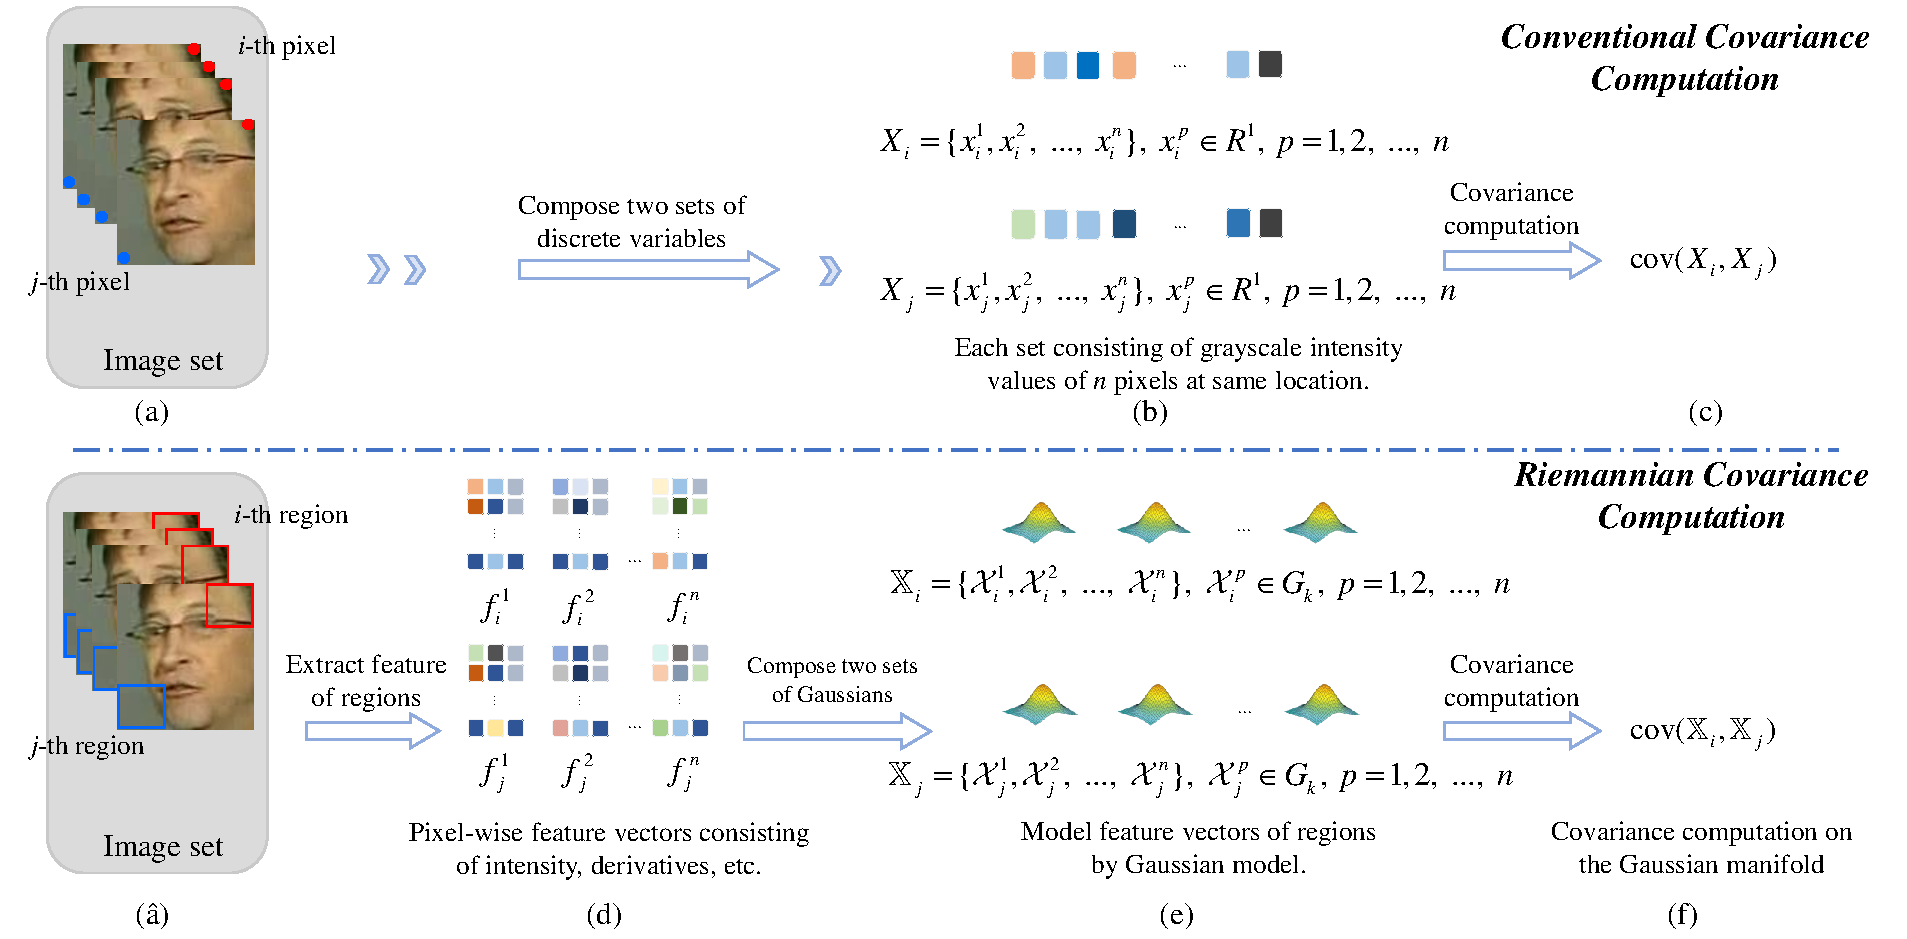
\includegraphics[width=0.99\linewidth]{Fig1.pdf} 
\end{center}
   \caption{ The flow chart of convetional covariance computation and Riemannian covariance computation. Top: conventional covariance computation. Bottom: Riemannian covariance computation. (a) input: image set. (b) two sets of discrete values, each set consisting of $n$ grayscale intensity values of $n$ pixels at the same location. (c) covariance via {Eq.(\ref{con_CovComputation})} between two sets. ($\hat{{\rm a}}$) input: image set. (d) pixel-wise features (position, first order gradients, etc.) of regions. (e) two sets of Gaussian models, each set consisting of $n$ Gaussian models of $n$ regions at the same location. (f) Riemamnnian covariance via {Eq.(\ref{Rie_CovComputation})} between two sets.}
\label{fig:short}
\end{figure*}
%- - - - - - - - - - - - - - - - - - - - - - - - - - - - - - - - - -
\subsection{Conventional covariance computation}
The covariance between two jointly distributed real-valued random variables $X$ and $Y$ with finite second moments is defined as the expected product of their deviations from their respective expected values\cite{dodge2006oxford}: cov($X$,$Y$) = E[($X$ - E($X$))($Y$ - E($Y$))], where E[$X$] is the expected value of $X$, also known as the mean of $X$. $X$ = $\{x_1,x_2,...,x_n\}$ and $Y$ = $\{y_1,y_2,...,y_n\}$ can also be sets of discrete scalar variables.
% where scalar values $x_p, y_p$ have equal probabilities $1/n$ for $p$ = $1,...,n$. 
Then the sample based covariance can be written in terms of the means E($X$) and E($Y$) as:
\begin{equation}
\label{con_CovComputation}
\mathop {\rm cov}(X,Y) = \frac{1}{n-1}\sum_{p=1}^n(x_p-{\rm E}(X))(y_p-{\rm E}(Y))
\end{equation} 
where ${\rm E}(X)=\frac{1}{n}{\sum_{p=1}^n}x_p$, ${\rm E}(Y)=\frac{1}{n}{\sum_{p=1}^n}y_p$.
%$x_p-{\rm E}(X)$ expresses the deviation from the corresponding expected value: ${\rm E}(X)$. Thus, the covariance is the expected product of the local difference vectors from their individual expected values. 
%- - - - - - - - - - - - - - - - - - - - - - - - - - - - - - - - - -
\subsection{Riemannian covariance computation}
	\indent Now let us assume that $\mathbb{X}$ = $\{\mathcal{X}_1,$$\mathcal{X}_2,$$...,$$\mathcal{X}_n \},$ $\mathcal{X}_p \in G_k$ and $\mathbb{Y}$ = $\{\mathcal{Y}_1,$$\mathcal{Y}_2,$$...,$$\mathcal{Y}_n \},$ $\mathcal{Y}_p \in G_k,$ $p=1,2,...,n$, are two sets of $n$ $k$-dimensional Gaussian models, which can be considered as the points on a Gaussian manifold \cite{wang2016towards}. Since the Euclidean operations are not applicable to the points on a Riemannian manifold, the operation of vector subtraction cannot be used for computing deviations from the expectation of Gaussian models. In \cite{faraki2015more}, Faraki et al. defined a Riemannian local difference vector (RieLDV) in terms of  geodesic distance and the gradient of geodesic distance functions. We adopt the idea here to define deviations on Gaussian manifold \cite{wang2016towards}. We propose the covariance computation on Gaussian manifold as:
\begin{equation}
\label{Rie_CovComputation}
\mathop {\rm cov}(\mathbb{X},\mathbb{Y}) = \frac{1}{n-1}\sum_{p=1}^n\zeta(\mathcal{X}_p,{\rm E}(\mathbb{X}))^T\,\zeta(\mathcal{Y}_p,{\rm E}(\mathbb{Y}))
\end{equation} 
where E($\mathbb{X}$) is the expected value of $\mathbb{X}$. The \emph{column vector} $\zeta(\mathcal{X}_p,{\rm E}(\mathbb{X}))$ is the RieLDV relative to ${\rm E}(\mathbb{X})$. The covariance on a Gaussian manifold is defined as the expected product of the Riemannian local difference vectors defined with respect to the expectation of the  Gaussian models. According to \cite{faraki2015more}, $\zeta(\mathcal{X}_p,{\rm E}(\mathbb{X}))$ has the following form:
\begin{equation}
\label{Rie_LDV}
\mathop \zeta(\mathcal{X}_p,{\rm E}(\mathbb{X})) = {\delta}(\mathcal{X}_p,{\rm E}(\mathbb{X}))\frac{\triangledown_{{\rm E}(\mathbb{X})}\delta^2(\mathcal{X}_p,{\rm E}(\mathbb{X}))}{\parallel\triangledown_{{\rm E}(\mathbb{X})}\delta^2(\mathcal{X}_p,{\rm E}(\mathbb{X}))\parallel}
\end{equation}
where $\delta$ is the geodesic distance on the curved manifold, and $\triangledown_{{\rm E}(\mathbb{X})}\delta^2(\mathcal{X}_p,{\rm E}(\mathbb{X}))$ \footnote{It should be noted that when computing the Riemannian gradient,  $\nabla_{X}Y$ does not signify the usual notation in Riemannian geometry, referring to the object $Y$ being covariantly differentiated along the vector field $X$. Instead, in {Eq.(\ref{Rie_LDV})} the lower index denotes the variables along which one differentiates.} is the gradient of the smooth distance function $\delta$ at point $E(\mathbb{X})$. \\
	\indent In the next section (Section 4), we introduce a sample representation in terms of a single Gaussian model and develop two methods for calculating the Riemannian local difference vector on the Gaussian manifold (RieLDV-G). Before concluding this section, we discuss how the conventional CovDs and Riemannian CovDs can be used to describe image sets.
%- - - - - - - - - - - - - - - - - - - - - - - - - - - - - - - - - -
\subsection{Riemannian CovDs for describing image set}
	\indent In the subsection, we follow the steps of Figure 1 to elaborate conventional CovDs and Riemannian CovDs for describing an image set. Given an image set with $n$ image samples, the final representation of an image set is a symmetric matrix obtained via Riemannian covariance computation between  regions at different locations instead of pixels. 
%- - - - - - - - - - - - - - - - - - - - - - - - - - - - - - - - - -
\subsubsection{Conventional CovDs}
	\indent Conventional CovDs for describing an image set generate representations via the covariance computation between the sets of discrete pixel values. Each set consists of $n$ grayscale pixel intensity values at the same image location. The conventional covariance matrix representation can be written as:
\begin{equation}
\label{con_CovDs}
\begin{split}
\mathop C = [C_{i,j}]{_{i,j=1,...,d}} \quad \quad\\
where \quad  {C_{i,j}}={\rm cov}(X_i,X_j)
\end{split}
\end{equation} 
where $d$ is the number of pixels in each image and $X_i$ denotes the set of grayscale intensity values at $i$-th pixel of $n$ image samples (Figure 1 step(b)).  $C_{i,j}$ is the covariance computed between two sets of grayscale values: $X_i$ and  $X_j$ (Figure 1 step(c)) defined  via {Eq.(\ref{con_CovComputation})}. The non-diagonal entry of the resulting covariance matrix $C$: $C_{i,j}$ is the covariance between $X_i$ and  $X_j$, which represents their respective correlation. The diagonal entries represent the variance of discrete values in each individual set.
%- - - - - - - - - - - - - - - - - - - - - - - - - - - - - - - - - -
\begin{table}
\renewcommand\arraystretch{1.15}
\centering
%\caption{\label{tab:overlapping}Algorithm 1 The proposed RieCovDs algorithm.}
%\vspace {2.5mm}
\scriptsize
%\tiny 
\resizebox{3.4in}{!}{
\begin{tabular}{m{6.5cm}}  
\hline 
$\textbf{Algorithm 1}$ The proposed RieCovDs algorithm\\
\hline
$\textbf{Input:}$ \\
$\qquad$ 	$\bullet$ An image set with $n$ images\\
$\textbf{Output:}$ \\
$\qquad$ 	$\bullet$ Riemannian CovDs for describing the image set\\
1: Divide the image into $D$ regions of the same size.\\
2: For the $i$-th  and $j$-th region of the image set (Figure 1 step($\hat{{\rm a}}$)), we first extract pixel-wise features of the regions (Figure 1 Step(d)).\\
3: Model feature vectors of the regions by a Gaussian model and obtain two sets of Gaussian models: $\mathbb{X}_i$ and $\mathbb{X}_j$ (Figure 1 Step(e)).\\
4: Calculate the covariance cov($\mathbb{X}_i$,$\mathbb{X}_j$) between $\mathbb{X}_i$ and $\mathbb{X}_j$ (Figure 1 Step(f)).\\
5: Generate the resulting covariance matrix $\mathbb{C}$ via {Eq.(\ref{Rie_CovDs})} . \\
\hline
\end{tabular}}
\end{table}
%- - - - - - - - - - - - - - - - - - - - - - - - - - - - - - - - - -
\subsubsection{Riemannian CovDs}
	Riemannian CovDs (RieCovDs) describe the correlations between regions instead of pixels and offer a more discriminative representation than the conventional CovDs for the task of image set classification. For the $i$-th and $j$-th region of the $n$ image samples (Figure 1 Step($\hat{{\rm a}}$)), we first extract pixel-wise features (positions, first order gradients, etc.) of the regions (Figure 1 Step(d)) and then use two sets of Gaussian models:  $\mathbb{X}_i$ =  $\{\mathcal{X}_i^1,$$\mathcal{X}_i^2,$$...,$$\mathcal{X}_i^n \}$ and $\mathbb{X}_j$ =  $\{\mathcal{X}_j^1,$$\mathcal{X}_j^2,$$...,$$\mathcal{X}_j^n \}$ (where $\mathcal{X}_i^p$ $\in$ $G_k$ denotes $i$-th region of $p$-th image) to represent them (Figure 1 Step(e)). The covariance cov($\mathbb{X}_i$,$\mathbb{X}_j$) (Figure 1 Step(f)) between $\mathbb{X}_i$ and $\mathbb{X}_j$ is then defined the  by Riemannian covariance computation ({Eq.(\ref{Rie_CovComputation})}). The resulting Riemannian CovDs descriptor of the image set is:
\begin{equation}
\label{Rie_CovDs}
\begin{split}
\mathop  \mathbb{C} = [\mathbb{C}_{i,j}]{_{i,j=1,...,D}} \quad \quad\\
where \quad  {\mathbb{C}_{i,j}}={\rm cov}(\mathbb{X}_i,\mathbb{X}_j)
\end{split}
\end{equation} 
In {Eq.(\ref{Rie_CovDs})}, $D$ is the number of regions in each image and $\mathbb{X}_i$ is the set of Gaussian models at the $i$-th region of the $n$ images. ${\mathbb{C}_{i,j}}$ denotes the covariance between the $i$-th  and $j$-th region. Algorithm 1 is referred to as RieCovDs.

%- - - - - - - - - - - - - - - - - - - - - - - - - - - - - - - - - -
\subsection{A comparison with other improved variants of the conventional CovDs for image set coding}
	The works in \cite{wang2015beyond,li2016spatial,chen2018Component} are the existing improved versions of the conventional CovDs for describing image sets, producing different representations. It is pertinent to elaborate their connections to and differences from the proposed approach.
 Wang et al.\cite{wang2015beyond} proposed an open framework based on the use of a kernel matrix defined over feature dimensions as a generic representation. This work used a non-linear kernel matrix as the representation that describes  similarities between pixels at different locations as a preamble to the conventional CovDs \cite{wang2012covariance}. Our work proposes to capture similarities between regions at different locations and uses  Gaussian models to represent them.
 Li et al.\cite{li2016spatial} extended the descriptive granularity of the covariance matrix from the traditional pixel-level to a more general patch-level. Though this work concentrates on the patch-level covariance computation, it is actually a sum-pooling form of the pixel-level covariances. Different from \cite{li2016spatial}, we extract pixel-level features instead of using intensity values and extend the covariance computation from Euclidean space to a Gaussian manifold. 
	Chen et al.\cite{chen2018Component} concentrated on similarities between  sub-image sets instead of the pixels and proposed a framework, which has been improved in \cite{chen2019more}, to generate a low-dimensional discriminative data representation for describing image sets. The main difference is that we describe the similarities between the regions at different locations via covariance computation on a Gaussian manifold instead of Log-Euclidean kernel \cite{wang2012covariance} on the SPD manifold.
%- - - - - - - - - - - - - - - - - - - - - - - - - - - - - - - - - - - - - - - - - - - - - - - - - - - - 

\section{Riemannian local difference vector on Gaussian manifold}
In this section, we first present a method of sample representation by a single Gaussian model. Then, we develop two methods that transform the problem of calculating Riemannian local difference vector on Gaussian manifold (RieLDV-G) to the task of calculating Riemannian local difference vector on SPD manifold (RieLDV-S). Finally, we introduce four frequently-used Riemannian metrics on SPD manifold and show how to calculate RieLDV-S by using these metrics.
%- - - - - - - - - - - - - - - - - - - - - - - - - - - - - - - - - -
\subsection{Gaussian model}
	\indent Consider a set of $N$ local features $F = \{ f_1,f_2,...,f_N | f_i \in R^k \}$. Using the maximum likehood method, we model their distribution via the following Gaussian model\cite{wang2016raid,wang2016towards}:
\begin{equation}
\label{eq5}
\begin{split}
\mathop \mathcal{N}(f_i|\mu,\Sigma) = \frac{{\rm exp}(-\frac{1}{2}(f_i - \mu)^T \Sigma^{-1} (f_i - \mu))}{\sqrt{(2\pi)^k{\rm det}(\Sigma)}}
\end{split}
\end{equation} 
where $\mu = \frac{1}{N}{\sum_{i=1}^N}{f_i}$ and $\Sigma = \frac{1}{N-1}{\sum_{i=1}^N}(f_i - \mu)^T(f_i - \mu)$ are the mean vector and covariance matrix, and det($\cdot$) denotes matrix determinant.\\
	\indent To calculate RieLDV-G, we develop two methods that transform the problem of RieLDV-G to the task of calculating RieLDV-S. In the first method, called directly calculated RieLDV-G (DE-RieLDV-G), we compute the local difference vector (LDV) relative to the  mean vector and RieLDV-S relative to the covariance matrix respectively, and then concatenate these two components as the final DE-RieLDV-G. The second, called indirectly calculated RieLDV-G (IE-RieLDV-G), maps $G_k$ via a Gaussian embdeding \cite{wang2016towards} into the space of SPD matrices, $S_{k+1}^{++}$, and then computes RieLDV-S. Finally, we use the resulting RieLDV-S as the IE-RieLDV-G. Table \ref{Abb_Of_RieLDV} summarizes the above abbreviations.
\begin{table}
\renewcommand\arraystretch{1.15}
\centering
\caption{\label{tab:overlapping}The Abbreviations of different types of Riemannian local difference vectors.}
\vspace {1.5mm}
\label{Abb_Of_RieLDV}
%\large
\normalsize 
%\scriptsize
%\tiny
\resizebox{3.2in}{!}{
\begin{tabular}{cccccc}
\hline 
Abbreviations					 	&Full Names		\\
\hline
RieLDV  							&Riemannian local difference vector\\
\multirow{2}*{RieLDV-S} 				&Riemannian local difference vector\\ & on SPD manifold	\\
\multirow{2}*{RieLDV-G} 				&Riemannian local difference vector\\ & on Gaussian manifold	\\
\multirow{2}*{DE-RieLDV-G}  			&Directly calculated Riemannian local difference\\ & vector on Gaussian manifold\\	
\multirow{2}*{IE-RieLDV-G}  			&Indirectly calculated Riemannian local difference\\ & vector on Gaussian manifold\\	
\hline
\end{tabular}}
\end{table}
%- - - - - - - - - - - - - - - - - - - - - - - - - - - - - - - - - -
\subsection{Calculating the Riemannian local difference vector on a Gaussian manifold} 
\vspace{8 pt}
\subsubsection{Directly calculated RieLDV-G (DE-RieLDV-G)}
	Let us consider a set of $n$ $k$-dimensional Gaussian models: $\mathbb{X} =  \{\mathcal{X}_1,\mathcal{X}_2,...,\\ \mathcal{X}_n|\mathcal{X}_i \sim \mathcal{N}(\mu_i,\Sigma_i)\}$. We compute RieLDV-G from the  mean vectors and covariance matrices. For the set of mean vectors $M = \{ \mu_1,\mu_2,...,\mu_n \}$, the set of local difference vectors in the Euclidean space is defined  by:
\begin{equation}
\label{LDV}
\begin{split}
\mathbb{L}_{E} = \{L_E^1,L_E^2,...,L_E^n \}  \qquad  \\
\end{split}
\end{equation} 
where $\ L_E^i = \mu_i - \tilde{\mu}$, and $\tilde{\mu} = \frac{1}{n}\sum_{p=1}^{n}\mu_p$. The set of covariance matrices $S = \{ \Sigma_1,\Sigma_2,...,\Sigma_n \}$ is considered as  a set of points on an SPD manifold. The set of Riemannian local difference vectors on the SPD manifold:
\begin{equation}
\label{RieLDV-S_k}
\begin{split}
\mathbb{L}_S = \{L_S^1,L_S^2,...,L_S^n \}  \qquad \\
\end{split}
\end{equation} 
where $\ L_S^i = \zeta(\Sigma_i,{\rm E}(S))$ is defined via {Eq.(\ref{Rie_LDV})}. ${\rm E}(S)$ is the Fr$\acute{\rm e}$chet mean of SPD matrices which will be introduced in Section 4.3. The set of DE-RieLDV-G is expressed as: 
\begin{equation}
\label{DE-RieLDV-G}
\begin{split}
\mathbb{L}_{DG} = \{L_{DG}^1,L_{DG}^2,...,L_{DG}^n \}  \qquad  \\
where \quad L_{DG}^i = [\alpha L_E^i;L_S^i] \quad \qquad   \\
\end{split}
\end{equation}
In {Eq.(\ref{DE-RieLDV-G})}, $L_{DG}^i$ is the concatenation of $L_E^i$ and $L_S^i$ with weight $\alpha > 0$. The relative effect of the local difference vectors in the Euclidean space and RieLDV-S on the SPD manifold on the resulting DE-RieLDV-G can be adjusted by $\alpha$. 

\subsubsection{Indirectly calculated RieLDV-G (IE-RieLDV-G)}
	\indent The space of $k$-dimensional Gaussian models is a Riemannian manifold. Let  $\mathcal{N}(\mu,\Sigma)$ be a Gaussian model with mean vector $\mu$ and covariance matrix $\Sigma$. Through a function $\Omega$, $\mathcal{N}(\mu,\Sigma)$ is mapped to an affine matrix  $\mathcal{A}$. Further, through the function $\Phi$, $\mathcal{A}$ is mapped to an SPD matrix $\mathcal{S}$. It is an element on the SPD manifold $S_{k+1}^{++}$. By these two functions $\Omega$ and $\Phi$, $\mathcal{N}(\mu,\Sigma)$ is uniquely designated as a $(k+1)\times(k+1)$ SPD matrix \cite{lovric2000multivariate}. With the consideration of the relative effect of the mean vector and the covariance matrix, Wang et al.\cite{wang2016towards} introduced a parameter $\beta > 0$ in the function $\Omega$:
\begin{equation}
\label{aff_Group}
\begin{split}
\mathop \Omega(\beta): \mathcal{N}(\mu,\Sigma) \to \mathcal{A} =  \left[  \begin{array}{cc}
      P &\beta\mu \\
      0^T & 1
    \end{array} \right] \\
\end{split}
\end{equation}
where $P$ is defined by the Cholesky factorization of $\Sigma$, i.e., $\Sigma = PP^T$. Accordingly, the representation of $\mathcal{N}(\mu,\Sigma)$ via the Gaussian manifold embedding \cite{wang2016towards} has the following form:
\begin{equation}
\label{Gauss_Embedding}
\mathop \mathcal{N}(\mu,\Sigma) \sim \mathcal{S} = \left[  \begin{array}{cc}
      \Sigma + {\beta}^2{\mu}{\mu}^T & \beta\mu \\
      \beta{\mu}^T & 1
    \end{array} \right]
\end{equation}
Accordingly, the space of $k$-dimensional Gaussian models has been embedded into SPD manifold $S_{k+1}^{++}$. For the set of $N$ $k$-dimensional Gaussian models: $\mathbb{X}$ =  $\{$$\mathcal{X}_1$,$\mathcal{X}_2$,...,$\mathcal{X}_n$$|$$\mathcal{X}_i$ $\sim$ $\mathcal{N}$($\mu_i$,$\Sigma_i$)$\}$, we have a set of their embedding matrices $\mathbb{S}$ =  $\{$$\mathcal{S}_1$,$\mathcal{S}_2$,...,$\mathcal{S}_n$$|$$\mathcal{S}_i$ $\in$ $S_{k+1}^{++}$$\}$. The set of IE-RieLDV-G is then given as: 
\begin{equation}
\label{IE-RieLDV-G}
\begin{split}
%\mathop{\arg\min}_{\theta}
\mathbb{L}_{IG} = \{L_{IG}^1,L_{IG}^2,...,L_{IG}^n \}  \quad \\
\end{split}
\end{equation}
where $L_{IG}^i$ is the resulting IE-RieLDV-G obtained by calculating the RieLDV-S of $i$-th embedded SPD matrix $\mathcal{S}_i$ on SPD manifold $S_{k+1}^{++}$.
%- - - - - - - - - - - - - - - - - - - - - - - - - - - - - - - - - -
\begin{table*}
\renewcommand\arraystretch{1.25}
\centering
\caption{\label{tab:overlapping}Metrics and associated gradients on the SPD manifold.}
\vspace {1.5mm}
\label{Gradient_OnSPD}
%\large
%\normalsize 
\scriptsize
\resizebox{4.5in}{!}{
\begin{tabular}{cccc}
\hline 
Metric  							&{$\delta^2$}$(X,Y)$   &$\triangledown_X\delta^2$	\\
\hline
AIRM \cite{pennec2006riemannian} 	&$\parallel$log($X^{-1/2}YX^{-1/2}$)$\parallel_F^2$			&2$X^{1/2}$log($X^{-1/2}YX^{-1/2}$)$X^{1/2}$\\

Stein \cite{sra2012new}			&log det($\frac{X+Y}{2}$) - $\frac{1}{2}$log det($XY$)			&$X(X+Y)^{-1}X-\frac{1}{2}X$\\

Jeffrey \cite{wang2004affine}		&$\frac{1}{2}$Tr($X^{-1}Y$) + $\frac{1}{2}$Tr($Y^{-1}X$) - $k$	&$\frac{1}{2}X(Y^{-1}-X^{-1}YX^{-1})X$\\

LEM	\cite{arsigny2007geometric} 	&$\parallel$log($Y$) - log($X$)$\parallel_F^2$				&$X$(log($X$)-log($Y$))+(log($X$)-log($Y$))$X$ \\	
\hline
\end{tabular}}
\end{table*}
%- - - - - - - - - - - - - - - - - - - - - - - - - - - - - - - - - -
\subsection{Calculating the Riemannian local difference vector on an SPD manifold}
	 In this section, we introduce Riemannian metrics on an SPD manifold, as well as the corresponding gradients and Riemannian means. Specifically, the expected value of a set of SPD matrices is expressed using the Fr$\acute{\rm e}$chet mean \cite{nielsen2013matrix}.
	 A real value $k \times k$ SPD matrix $X$ $\in$ $S_k^{++}$ satisfies $v^TXv$$\ge$0 for all non-zero $v$ $\in$ $R^k$. The SPD manifold $S_k^{++}$ can be considered as the interior of a convex cone in the $k$($k$+1)/2-dimensional Euclidean space which is a non-linear Riemannian manifold \cite{harandi2014manifold,harandi2018dimensionality}. The Affine Invariant Riemannian Metric (AIRM) is the mostly studied Riemannian metric on SPD manifolds \cite{pennec2006riemannian}. Beside AIRM, Log-Euclidean Metric (LEM) \cite{arsigny2007geometric} and two types of Bregman divergence \cite{kulis2009low}, namely Stein \cite{sra2012new} and Jeffrey \cite{wang2004affine} divergence, are also widely used to analyze SPD matrices. Given two SPD matrices $X$, $Y$ $\in$ $S_k^{++}$, their distance computed via these four metrics ($\delta_A$, $\delta_L$, $\delta_S$, $\delta_J$) is described in Table 2.  The gradients of $\delta_A^2$ and $\delta_L^2$ are reported in \cite{pennec2006riemannian} and \cite{arsigny2007geometric} 
respectively, and the gradients of $\delta_S^2$ and $\delta_J^2$ are derived  in \cite{cherian2013jensen}. The gradients required for calculating RieLDV-S via {Eq.(\ref{Rie_LDV})} are summarized in Table \ref{Gradient_OnSPD}. 

%- - - - - - - - - - - - - - - - - - - - - - - - - - - - - - - - - -
%\begin{bfseries}Definition 1\end{bfseries} \emph{The cost function of Fr$\acute{\rm e}$chet mean \cite{nielsen2013matrix} for a set of points ${\{x_i\}}_{i=1}^{m}$ is:}
	Let us consider the following cost function for a set of points ${\{x_i\}}_{i=1}^{m}$. The Fr$\acute{\rm e}$chet mean \cite{nielsen2013matrix} is then defined as the local minimizer of this cost function.
\begin{equation}
\label{fre_Mean}
\begin{split}
c^* = \mathop{\arg\min}_{c}\sum_{i=1}^{m}\delta^2(c,x_i)  \\
\end{split}
\end{equation}
%the Fr$\acute{\rm e}$chet mean \cite{nielsen2013matrix} is the local minimizer of the above cost function which is the sum of squared distances.\\
For a set of SPD matrices ${\{X_i\}}_{i=1}^{m} \in S_{k}^{++} $, the Fr$\acute{\rm e}$chet mean with AIRM and Stein divergence are obtained by an iterative approach \cite{pennec2006riemannian,cherian2013jensen}. An estimate of the Fr$\acute{\rm e}$chet mean with AIRM at the $t+1$ step is obtained \cite{pennec2006riemannian}:
\begin{equation}
\label{eq14}
{\mu}_{t+1} = \mu_{t}^{\frac{1}{2}}\exp(\frac{1}{m}\sum_{i=1}^{m}\log(\mu_{t}^{-\frac{1}{2}}{X_i}\mu_{t}^{-\frac{1}{2}}))\mu_{t}^{\frac{1}{2}}
\end{equation} 
where log($\cdot$) and exp($\cdot$) are the matrix logarithm and matrix exponential respectively. For the Stein divergence, the estimate at iteration $t+1$ is given as:
\begin{equation}
\label{eq15}
{\mu}_{t+1} = \lbrack \frac{1}{m}\sum_{i=1}^{m}(\frac{X_i+\mu_t}{2})^{-1} \rbrack^{-1}
\end{equation} 
The proof is presented in \cite{cherian2013jensen}. The Fr$\acute{\rm e}$chet mean with Jeffrey divergence is obtained analytically as \cite{faraki2015more}:
\begin{equation}
\label{eq16}
{\mu} = P^{-\frac{1}{2}}(P^{\frac{1}{2}}QP^{\frac{1}{2}})^{\frac{1}{2}} P^{-\frac{1}{2}}
\end{equation} 
where $P = \sum_{i}X_{i}^{-1}$ and $Q = \sum_{i}X_{i}$. The Fr$\acute{\rm e}$chet mean with LEM is obtained analytically as \cite{arsigny2007geometric}:
\begin{equation}
\label{eq17}
{\mu} = \exp(\frac{1}{m}\sum_{i=1}^{m}\log(X_i))
\end{equation} 
For more details on the Fr$\acute{\rm e}$chet mean with Jeffrey divergence and LEM, the interested readers
can refer to \cite{faraki2015more,arsigny2007geometric}.
%- - - - - - - - - - - - - - - - - - - - - - - - - - - - - - - - - - - - - - - - - - - - - - - - - - - - - - - - - - - - - - - - - - - - - - - - - - - -
\section{Experiments and Analysis}
	 This section presents the results of  comparative experiments on datasets relating to the task of image set classification. The four datasets are Cambridge hand-gesture \cite{kim2009canonical}, ETH-80 \cite{leibe2003analyzing}, Virus \cite{kylberg2011virus} and MDSD \cite{shroff2010moving} datasets respectively.
%- - - - - - - - - - - - - - - - - - - - - - - - - - - - - - - - - -
\subsection{Datasets and settings}
	\indent Our first experiment involves the task of hand gesture recognition. We use the Cambridge hand-gesture dataset \cite{kim2009canonical} that contains nine categories of samples and nine hundred image sets. For each class twenty image sets are chosen randomly as training samples and the remaining eighty image sets are reserved for testing. 
	
	In the ETH-80 dataset \cite{leibe2003analyzing}, there are eight categories of samples and eighty image sets. For each class, five image sets are randomly chosen for training and the remaining five image sets are used for testing. 
	
	In the Virus cell dataset \cite{kylberg2011virus}, there are fifteen categories of samples and 100 gray images in each category. We divide the images of each category equally into five different image sets and obtain seventy-five image sets. For each class, three image sets are randomly chosen as training samples and the remaining two image sets for testing. 
	
	The MDSD dataset \cite{shroff2010moving} has been used for the task of dynamic scene classification. Following the settings in \cite{sun2017learning}, we test the method based on the protocol of seventy-thirty-ratio (STR) which chooses seven videos for training and three videos for testing in each class. We divide each video into about 60 clips.  $f_i^p$ (in figure 1 Step(d)) represents the pixel-wise features of frames at the $i$-th region of the $p$-th video clip.
	 
In our experiment, an 11-dimensional local feature vector is extracted from the colour image $I$ as follows:
\begin{equation}
\begin{split}
\label{color_Feature}
\mathop F(x,y) = [x,y,I_R(x,y),\lvert\frac{\partial{I_R}}{\partial{x}}\rvert,\lvert\frac{\partial{I_R}}{\partial{y}}\rvert,I_G(x,y),\\
 \lvert\frac{\partial{I_G}}{\partial{x}}\rvert,\lvert\frac{\partial{I_G}}{\partial{y}}\rvert,I_B(x,y),\lvert\frac{\partial{I_B}}{\partial{x}}\rvert,\lvert\frac{\partial{I_B}}{\partial{y}}\rvert]
\end{split}
\end{equation} 
The first two components are the $x$ and $y$ coordinates of a pixel $(x,y)$. $I_R(x,y)$, $I_G(x,y)$, $I_B(x,y)$ represent the corresponding color information and $\lvert\frac{\partial{I_R}}{\partial{x}}\rvert$, $\lvert\frac{\partial{I_R}}{\partial{y}}\rvert$, $\lvert\frac{\partial{I_G}}{\partial{x}}\rvert$, $\lvert\frac{\partial{I_G}}{\partial{y}}\rvert$, $\lvert\frac{\partial{I_B}}{\partial{x}}\rvert$, $\lvert\frac{\partial{I_B}}{\partial{y}}\rvert$ capture the first order gradients of the corresponding colour information. For the gray image (In Virus dataset \cite{kylberg2011virus}), the 5-dimensional feature vectors are extracted by:
\begin{equation}
\begin{split}
\label{gray_Feature}
\mathop F(x,y) = [x,y,I(x,y),\lvert\frac{\partial{I}}{\partial{x}}\rvert,\lvert\frac{\partial{I}}{\partial{y}}\rvert]
\end{split}
\end{equation} 
where the last three dimensions are the grayscale intensity and the corresponding first order gradients.

	For our proposed RieCovDs, the size of the image is 240$\times$320 on the Cambridge and MDSD datasets, 256$\times$256 on the ETH-80 dataset, and 40$\times$40 on the Virus dataset. We use the sliding window method to obtain the regions at different locations. The size of the sliding window is 60$\times$80, 32$\times$32, 5$\times$5, 60$\times$80 on the Cambridge, ETH-80, Virus and MDSD datasets. The step size is `30', `28', `5', `20' pixels in the horizontal direction and `40', `28', `5', `30' pixels in the vertical direction for these four datasets respectively. We set parameter $\alpha$ in {Eq.(\ref{DE-RieLDV-G})} to be 0.2, 0.9, 1, 0.3 for the four datasets respectively and set $\beta$ in {Eq.(\ref{aff_Group})} to be 0.7, 0.6, 0.4, 0.9 respectively. For each RieLDV-G $\mathbb{L}_G$, the normalization is performed using the transfer function: $sign(\mathbb{L}_G)\sqrt{|\mathbb{L}_G|}$, where $|\cdot|$ denotes an absolute value operation. The gradient of the geodesic distance function at $X$: $\triangledown_X\delta^2$, is normalized  by: $X^{-1/2}\triangledown_X\delta^2X^{-1/2}$.   
%- - - - - - - - - - - - - - - - - - - - - - - - - - - - - - - - - -
\subsection{Comparison with the conventional CovDs}
	For the comparative experiments with the conventional CovDs \cite{wang2012covariance}, five algorithms are used to demonstrate the merits of our proposed RieCovDs. They include four nearest neighbor (NN) algorithms based on the above four Riemannian metrics on the SPD manifold, and the well-known SVM classifier \cite{chang2011libsvm}. The different classifiers tested in our experiments are referred to as: \\
\begin{bfseries}NN-AIRM:\end{bfseries} AIRM based Nearest Neighbor classifier.\\
\begin{bfseries}NN-Stein:\end{bfseries} $S$ divergence based Nearest Neighbor classifier.\\
\begin{bfseries}NN-Jeffrey:\end{bfseries} $J$ divergence based Nearest Neighbor classifier.\\
\begin{bfseries}NN-LEM:\end{bfseries} LEM based Nearest Neighbor classifier.\\
\begin{bfseries}Ker-SVM:\end{bfseries} Log-Euclidean Kernel \cite{wang2012covariance} based SVM classifier.

	Here, Ker-SVM is a one-vs-all SVM classifier \footnote{http://www.peihuali.org/publications/RAID-G/RIAD-G\_V1.zip} implemented by Wang et al. Following \cite{wang2012covariance}, we regularize the conventional covariance matrix by: $C^{*} = C + \lambda\times Tr(C)I$ and set $\lambda$ = $10^{-3}$ typically. If the minimum eigenvalue of the representation computed by our proposed RieCovDs is less than $10^{-9}$, then we regularize it by setting $\lambda$ = $10^{-9}$. For the covariance matrices of the regions and the resulting representation via the Gaussian embedding, we regularize them in a similar manner. The different descriptors in this paper are referred to as:
	
\begin{bfseries}CovDs:\end{bfseries} Image set repesented by conventional CovDs \cite{wang2012covariance}.\\
\begin{bfseries}RieCovDs-A-DE/IE:\end{bfseries} Riemannian CovDs via DE-RieLDV-G/IE-RieLDV-G and using AIRM to compute the component of RieLDV-S.\\
\begin{bfseries}RieCovDs-L-DE/IE:\end{bfseries} Riemannian CovDs via DE-RieLDV-G/IE-RieLDV-G and using LEM to compute the component of RieLDV-S.\\
\begin{bfseries}RieCovDs-S-DE/IE:\end{bfseries} Riemannian CovDs via DE-RieLDV-G/IE-RieLDV-G and using $S$ divergence to compute the component of RieLDV-S.\\
\begin{bfseries}RieCovDs-J-DE/IE:\end{bfseries} Riemannian CovDs via DE-RieLDV-G/IE-RieLDV-G and using $J$ divergence to compute the component of RieLDV-S.\\
\begin{table*}
\renewcommand\arraystretch{1.1}
\centering
\caption{\label{tab:overlapping} \upshape A comparison  of the conventional CovDs and RieCovDs using different classifiers.}
\vspace {1.5mm}
\label{CovDs_Compare}
%\Huge
%\huge
\LARGE
%\Large
%\large
%\normalsize 
%\scriptsize
%\tiny   
\resizebox{4.3in}{!}{
\begin{tabular}{|c|c|c|c|c|c|c|}
\hline 
Methods 	&Descriptors	&Cambridge\cite{kim2009canonical}   &ETH-80\cite{leibe2003analyzing}  &Virus\cite{kylberg2011virus}  &MDSD\cite{shroff2010moving}  \\
\hline
\multirow{5}*{NN-AIRM} 
&CovDs \cite{wang2012covariance}		&55.29$\pm$2.53			&77.05$\pm$4.85			&27.00$\pm$4.12 		&13.90$\pm$4.30\\
\cdashline{2-6}[1pt/2pt]
&RieCovDs-A-DE/IE		&94.51$\pm$0.96 / 94.49$\pm$0.96  				&93.30$\pm$3.84 / 94.95$\pm$3.71  		
					&52.80$\pm$5.82 / 72.50$\pm$6.27 				&33.82$\pm$6.45 / 31.33$\pm$6.09\\
\cdashline{2-6}[1pt/2pt]
&RieCovDs-S-DE/IE		&94.48$\pm$0.93 / 94.36$\pm$0.96  				&91.70$\pm$3.33 / 94.30$\pm$3.63  
					&51.23$\pm$5.31 / 72.00$\pm$6.32  				&27.41$\pm$6.01 / 32.54$\pm$6.42\\
\cdashline{2-6}[1pt/2pt]
&RieCovDs-J-DE/IE		&94.33$\pm$0.91 / 94.54$\pm$1.04  				&90.83$\pm$3.26 / 91.92$\pm$3.71  
					&55.07$\pm$4.58 / 72.93$\pm$6.48  				&27.51$\pm$5.73 / 24.79$\pm$5.69\\
\cdashline{2-6}[1pt/2pt]
&RieCovDs-L-DE/IE		&95.00$\pm$0.90 / 95.09$\pm$0.84  				&93.45$\pm$3.79 / 93.85$\pm$3.54  
					&52.80$\pm$5.52 / 72.30$\pm$6.26  				&34.74$\pm$6.31 / 31.18$\pm$6.05\\
\hline
\multirow{5}*{NN-Stein} 
&CovDs \cite{wang2012covariance}		&43.57$\pm$2.76			&65.27$\pm$5.18			&25.80$\pm$4.68 		&13.44$\pm$4.39\\
\cdashline{2-6}[1pt/2pt]
&RieCovDs-A-DE/IE		&92.18$\pm$1.16 / 93.65$\pm$0.89  				&93.25$\pm$3.85 / 94.58$\pm$3.64  
					&46.07$\pm$4.33 / 72.90$\pm$6.71  				&34.67$\pm$6.42 / 31.08$\pm$6.22\\
\cdashline{2-6}[1pt/2pt]
&RieCovDs-S-DE/IE		&92.54$\pm$1.13 / 93.68$\pm$0.89  				&91.65$\pm$3.00 / 94.47$\pm$3.56  
					&45.97$\pm$4.43 / 72.83$\pm$6.69  				&27.49$\pm$6.36 / 32.21$\pm$6.31\\
\cdashline{2-6}[1pt/2pt]
&RieCovDs-J-DE/IE		&89.78$\pm$1.37 / 93.24$\pm$0.97 				&90.93$\pm$3.17 / 92.02$\pm$3.55  
					&47.53$\pm$4.78 / 74.37$\pm$6.59  				&28.64$\pm$5.82 / 25.41$\pm$6.23\\
\cdashline{2-6}[1pt/2pt]
&RieCovDs-L-DE/IE		&93.00$\pm$1.00 / 93.90$\pm$0.97 	 			&92.53$\pm$3.58 / 94.03$\pm$3.44  
					&46.87$\pm$5.56 / 74.53$\pm$6.47  				&34.74$\pm$6.77 / 30.13$\pm$5.87\\
\hline
\multirow{5}*{NN-Jeffrey} 
&CovDs \cite{wang2012covariance}		&83.80$\pm$1.51			&87.73$\pm$4.91			&32.20$\pm$5.71 		&19.08$\pm$4.99\\
\cdashline{2-6}[1pt/2pt]
&RieCovDs-A-DE/IE		&89.04$\pm$1.30 / 89.70$\pm$1.27  				&93.50$\pm$3.62 / 95.12$\pm$3.85  
					&61.67$\pm$7.07 / 61.93$\pm$6.29  				&32.36$\pm$6.04 / 33.74$\pm$6.37\\
\cdashline{2-6}[1pt/2pt]
&RieCovDs-S-DE/IE		&89.89$\pm$1.19 / 90.02$\pm$1.24  				&92.52$\pm$3.53 / 94.35$\pm$3.70  
					&60.90$\pm$6.48 / 61.93$\pm$6.23  				&27.36$\pm$5.94 / 32.56$\pm$6.54\\
\cdashline{2-6}[1pt/2pt]
&RieCovDs-J-DE/IE		&86.11$\pm$1.80 / 88.11$\pm$1.40  				&90.57$\pm$3.67 / 91.68$\pm$3.84 
					&61.73$\pm$6.47 / 61.77$\pm$6.29  				&25.15$\pm$5.45 / 20.33$\pm$5.09\\
\cdashline{2-6}[1pt/2pt]
&RieCovDs-L-DE/IE		&89.11$\pm$1.25 / 89.65$\pm$1.19 		 		&93.45$\pm$3.62 / 93.70$\pm$3.83  
					&63.67$\pm$6.35 / 63.37$\pm$6.61  				&33.69$\pm$6.07 / 33.51$\pm$6.26\\
\hline
\multirow{5}*{NN-LEM} 
&CovDs \cite{wang2012covariance}		&71.17$\pm$1.87			&81.85$\pm$5.75			&26.30$\pm$4.69 		&14.82$\pm$4.72\\
\cdashline{2-6}[1pt/2pt]
&RieCovDs-A-DE/IE		&94.60$\pm$0.95 / 94.38$\pm$0.96  				&93.03$\pm$3.71 / 94.80$\pm$3.58  
					&51.93$\pm$5.08 / 71.50$\pm$6.35  				&34.23$\pm$6.32 / 32.54$\pm$6.25\\
\cdashline{2-6}[1pt/2pt]
&RieCovDs-S-DE/IE		&94.59$\pm$0.90 / 94.34$\pm$0.92  				&91.15$\pm$3.25 / 94.10$\pm$3.58  
					&51.07$\pm$5.36 / 70.67$\pm$6.82		  		&29.79$\pm$6.09 / 33.69$\pm$6.47\\
\cdashline{2-6}[1pt/2pt]
&RieCovDs-J-DE/IE		&94.51$\pm$0.92 / 94.30$\pm$1.05  				&90.88$\pm$2.98 / 91.63$\pm$4.16 
					&52.17$\pm$5.43 / 72.00$\pm$6.80  				&27.28$\pm$5.58 / 26.31$\pm$5.86\\
\cdashline{2-6}[1pt/2pt]
&RieCovDs-L-DE/IE		&95.08$\pm$0.92 / 94.76$\pm$0.90  				&92.90$\pm$3.65 / 93.93$\pm$3.47  
					&53.37$\pm$5.29 / 73.00$\pm$6.44  				&34.10$\pm$6.24 / 33.74$\pm$6.44\\
\hline
\multirow{5}*{Ker-SVM} 
&CovDs \cite{wang2012covariance}		&91.67$\pm$1.10			&92.48$\pm$5.08			&66.57$\pm$5.79 		&35.38$\pm$6.25\\
\cdashline{2-6}[1pt/2pt]
&RieCovDs-A-DE/IE		&96.89$\pm$0.75 / {\bfseries 96.93$\pm$0.76}  		&98.25$\pm$2.53 / {\bfseries 98.55$\pm$2.17}  
					&73.63$\pm$6.01 / 80.60$\pm$5.79  				&46.92$\pm$5.87 / 45.51$\pm$6.43\\
\cdashline{2-6}[1pt/2pt]
&RieCovDs-S-DE/IE		&96.36$\pm$0.81 / 96.11$\pm$0.95  				&97.87$\pm$2.26 / 98.00$\pm$2.61  
					&70.30$\pm$6.16 / {\bfseries 82.17$\pm$5.81}  		&40.67$\pm$6.44 / 42.26$\pm$6.28\\
\cdashline{2-6}[1pt/2pt]
&RieCovDs-J-DE/IE		&94.20$\pm$0.96 / 94.09$\pm$1.00 				&94.53$\pm$2.90 / 96.52$\pm$2.58  
					&78.07$\pm$6.01 / 77.73$\pm$7.09  				&38.59$\pm$5.31 / 37.97$\pm$6.48\\
\cdashline{2-6}[1pt/2pt]
&RieCovDs-L-DE/IE		&96.86$\pm$0.75 / 96.70$\pm$0.83  				&98.35$\pm$2.44 / 98.00$\pm$2.86  
					&72.70$\pm$6.04 / 78.37$\pm$5.29  				&{\bfseries 47.21$\pm$5.92} / 45.38$\pm$6.16\\
\hline
\end{tabular}}
\end{table*}
	
	Table \ref{CovDs_Compare} shows the average recognition accuracies and standard deviations of different descriptors with different classifiers. The advantage of our proposed RieCovDs is evident from the results obtained using the same classifier. This shows the effectiveness of our proposed RieCovDs. Ker-SVM achieves the best recognition accuracy of $96.93\%$, $98.55\%$, $82.17\%$, $47.21\%$ with RieCovDs-A-IE, RieCovDs-A-IE, RieCovDs-S-IE, RieCovDs-L-DE on the four datasets respectively.
	
	In the next sub-section, we consider the results of the best classifier, namely the Ker-SVM classifier, and compare them with state-of-the-art (SOTA) methods, which include SOTA classifiers and other improved versions of the conventional CovDs for the task of image set classification.
%- - - - - - - - - - - - - - - - - - - - - - - - - - - - - - - - - -
\subsection{Comparison with SOTA methods}
	\indent In this section, we compare with the SOTA classifiers including Covariance Discriminative Learning (COV-LDA, COV-PLS) \cite{wang2012covariance}, Log-Euclidean Kernels for Sparse Representation (LogEKSR.Pol, LogEKSR.Exp and LogEKSR.Gau) \cite{li2013log}, SPD Manifold Learning based on LEM (SPDML-LEM) \cite{harandi2018dimensionality}, Log-Euclidean Metric Learning (LEML, LEML+COV-LDA, LEML+COV-PLS) \cite{huang2015log}, Riemannian Network for SPD Matrix Learning (SPDNet) \cite{huang2017riemannian} and Multiple Manifolds Metric Learning (MMML) \cite{wang2018multiple}. For these methods, we first resize all images to 20$\times$20,  and then use the intensity values as their features. The latent dimensions in COV-LDA/COV-PLS are set to $c-1$/$c+1$, where $c$ is the number of classes. For these SOTA classifiers, we report the best accuracies by searching over their various parameter settings.
	
	The methods in \cite{wang2015beyond,li2016spatial,chen2018Component} are the other improved versions of the conventional CovDs for describing image sets. For the comparative experiments with SOTA descriptors, we use the accuracies of the Ker-SVM classifier tested on these representations as the final results. To generate the descriptor in \cite{wang2015beyond}, named CovDs-B \footnote{https://www.uow.edu.au/~leiw/} in this paper, we use the kernel matrix representation obtained with  the RBF kernel as it has been shown to achieve a better accuracy \cite{wang2015beyond}. To generate the descriptor in \cite{chen2018Component}, named CovDs-C \footnote{https://github.com/Kai-Xuan/ComponentSPD/} , all images are resized to 24$\times$24 and sub-image sets are obtained by a 6$\times$6 sliding window with the spatial step of 2 pixels for CG, ETH-80 and MDSD datasets, and spatial step of 3 pixels for the Virus dataset. For the method in \cite{li2016spatial}, named CovDs-P in this paper, the sliding window size and step size are the same as the settings of CovDs-C on the corresponding dataset of patch-level images. The CovDs-B \cite{wang2015beyond} and CovDs-P \cite{li2016spatial} descriptors are regularized  as the conventional CovDs.\\
%------------------------------------------------
\begin{table*}
\renewcommand\arraystretch{1.1}
\centering
\caption{\label{tab:overlapping}Average recognition accuracies and standard deviations of different classifiers.}
\vspace {1.5mm}
\label{SOTA_Compare}
%\Large
\normalsize 
%\small
%\footnotesize
%\tiny  
\resizebox{4.7in}{!}{
\begin{tabular}{cccccc}
\hline 
Methods	&Cambridge \cite{kim2009canonical}  	&ETH-80 \cite{leibe2003analyzing}    &Virus \cite{kylberg2011virus} 	&MDSD \cite{shroff2010moving}\\
\hline
COV-LDA \cite{wang2012covariance}		&90.25$\pm$1.64	 	&93.95$\pm$4.30		&46.40$\pm$5.76		&34.10$\pm$5.90		\\
COV-PLS \cite{wang2012covariance}		&88.95$\pm$1.26		&94.23$\pm$4.63		&62.84$\pm$5.99		&36.74$\pm$5.62		\\
LogEKSR.Pol \cite{li2013log}			&92.32$\pm$1.19		&95.00$\pm$3.28		&58.53$\pm$6.54		&36.23$\pm$6.81		\\
LogEKSR.Exp \cite{li2013log}			&92.23$\pm$1.18		&95.10$\pm$3.20		&59.03$\pm$6.38		&36.59$\pm$6.88		\\
LogEKSR.Gau \cite{li2013log}			&92.33$\pm$1.18		&95.18$\pm$3.30		&61.80$\pm$6.35		&37.95$\pm$6.83		\\
LEML	\cite{huang2015log}				&88.18$\pm$1.29		&93.05$\pm$3.31		&33.00$\pm$5.70		&25.97$\pm$6.79		\\
LEML+COV-LDA \cite{huang2015log}		&89.09$\pm$1.63		&95.35$\pm$3.50		&58.03$\pm$5.84		&31.92$\pm$6.44		\\
LEML+COV-PLS \cite{huang2015log}		&86.36$\pm$1.35		&95.83$\pm$3.04		&59.40$\pm$6.22		&35.90$\pm$6.98		\\
SPDML-LEM \cite{harandi2018dimensionality}	&84.03$\pm$1.04		&90.63$\pm$4.19		&49.37$\pm$7.46		&24.23$\pm$4.47		\\
SPDNet \cite{huang2017riemannian}		&92.03$\pm$1.46		&95.50$\pm$3.69		&59.70$\pm$4.58		&33.76$\pm$5.04		\\
MMML \cite{wang2018multiple}			&92.87$\pm$1.39		&95.28$\pm$3.80		&51.13$\pm$7.60		&31.95$\pm$6.26		\\
\cdashline{1-6}[1.0pt/1.5pt]
Ker-SVM + CovDs-B \cite{wang2015beyond}	&92.31$\pm$1.13		&94.18$\pm$3.69		&73.77$\pm$5.82		&37.79$\pm$5.76		\\
Ker-SVM + CovDs-P \cite{li2016spatial}	&94.34$\pm$1.02		&94.52$\pm$3.64		&75.40$\pm$6.01		&35.54$\pm$6.47		\\
Ker-SVM + CovDs-C \cite{chen2018Component} &93.81$\pm$0.91		&95.45$\pm$2.85		&53.63$\pm$6.80		&38.08$\pm$6.05		\\
\textbf{Ker-SVM + RieCovDs(Ours)}		&\textbf{96.93$\pm$0.76}	&\textbf{98.55$\pm$2.17}	&\textbf{82.17$\pm$5.81}	&\textbf{47.21$\pm$5.92}\\
\hline
\end{tabular}}
\end{table*}
	
	As shown in Table \ref{SOTA_Compare}, the experimental results demonstrate the superior performance of our method, measured in terms of recognition accuracy. The advantages of our methods are very clear on the Virus and MDSD datasets, where image samples contain a large amount of noise. Our method achieves the best recognition accuracies with low standard deviations on the four datasets.
%- - - - - - - - - - - - - - - - - - - - - - - - - - - - - - - - - -
\begin{figure}
\begin{center}
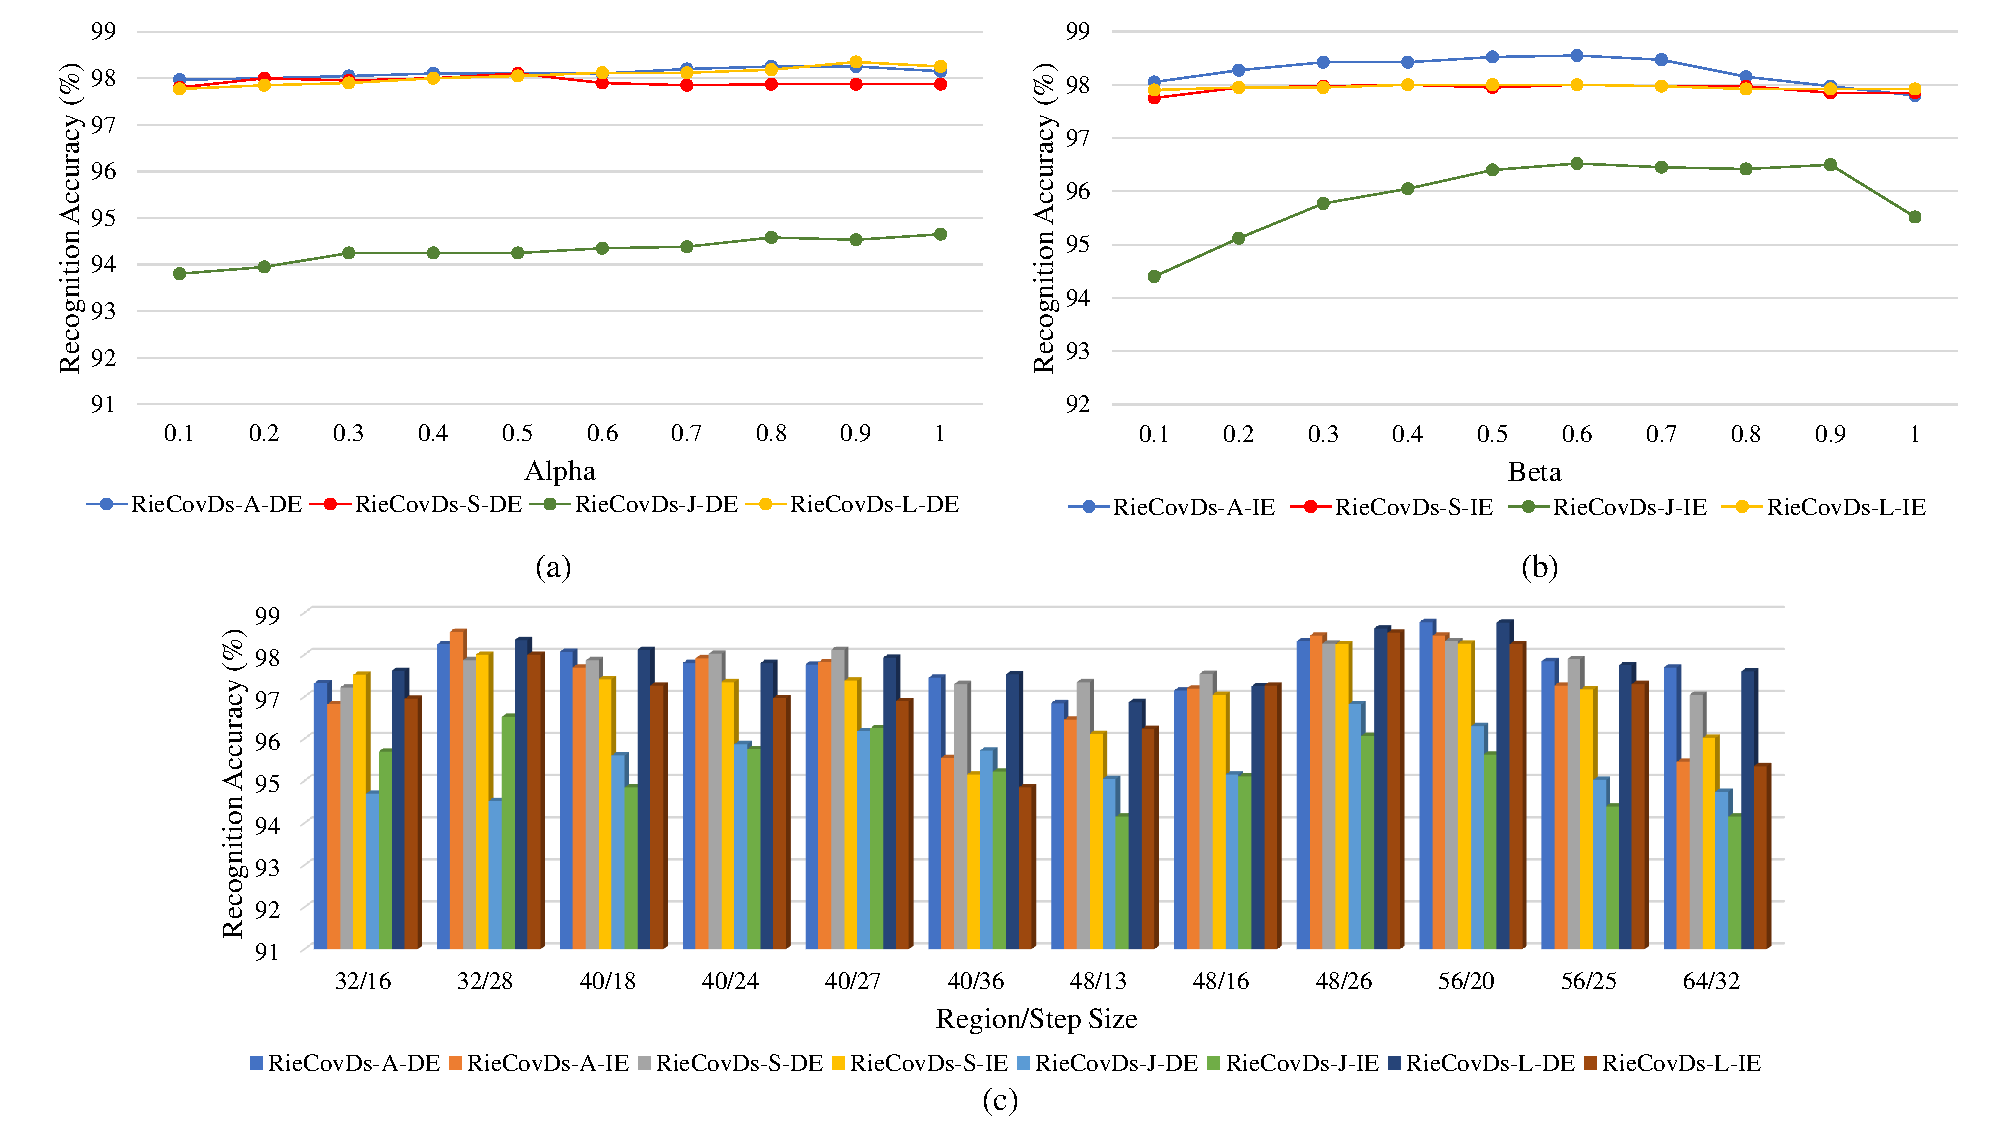
\includegraphics[width=0.99\linewidth]{Res_ETH.pdf} 
\end{center}
   \caption{The effect of balance parameter $\alpha$ in Eq.(\ref{DE-RieLDV-G}), $\beta$ in Eq.(\ref{aff_Group}) and different region/step sizes on ETH-80 dataset. }
\label{fig:short}
\end{figure}
%- - - - - - - - - - - - - - - - - - - - - - - - - - - - - - - - - -
\subsection{Ablation study}
	The results in Table \ref{CovDs_Compare} and Table \ref{SOTA_Compare} demonstrate  the superior performance of our proposed RieCovDs  method. 
	%has been demonstrated. This can be mainly attributed to the more comprehensive information being captured by  regions than pixels \cite{wang2012covariance,wang2015beyond}. For the covariance computation, we developed two methods to calculate RieLDV on the Gaussian manifold  instead of the subtraction operation in the Euclidean space \cite{wang2012covariance,li2016spatial}. 
	 The results have been obtained by fine tuning the various meta parameters of the method, namely the balance parameter $\alpha$ in Eq.(\ref{DE-RieLDV-G}), $\beta$ in Eq.(\ref{aff_Group}), the sliding window/step size, the normalization of RieLDV-G $\mathbb{L}_G$ and gradient $\triangledown_X\delta^2$. In order to validate their contributions, we investigate the sensitivity of the recognition accuracies produced by the Ker-SVM classifier on ETH-80 dataset \cite{leibe2003analyzing} to changes in these parameters. The results of RieCovDs with various $\alpha$ and $\beta$ are illustrated in Figure 2 (a) and (b). Figure 2 (c) shows the effect of region size and step size on the recognition accuracies. The horizontal ordinate is in the form of `$a/b$', which means that the sliding window size is $a\times a$ and step size is $b$ pixels in both two directions. The results in figure 2 show that our proposed method is more sensitive to the sliding window/step size than the balance parameter $\alpha$ and  $\beta$.
	 
	The effect of the four kinds of data preprocessing on Riemannian covariance was measured by comparing the results of the following variants: keeping the original form of RieLDV-G and gradient (KORG), normalizing only  RieLDV-G (NORR), normalizing only gradient (NORG), normalizing RieLDV-G and gradient (NORR+NORG). The results are shown in Table \ref{Normalization_Compare}. From the results, we can conclude that the normalization of RieLDV-G and gradient are the most important steps in the computation of Riemannian covariance.
%------------------------------------------------
\begin{table*}
\renewcommand\arraystretch{0.9}
\centering
\caption{\label{tab:overlapping} The effect of four kinds of data preprocessing on the Riemannian covariance.}
\vspace {1.5mm}
\label{Normalization_Compare}
%\Large
%\normalsize 
\small
%\footnotesize
%\tiny  
\resizebox{4.2in}{!}{
\begin{tabular}{cccccc}
\hline 
Descriptors			&KORG  	&NORR    &NORG 	&NORR+NORG\\
\hline
RieCovDs-A-DE			&92.48$\pm$3.92	 	&94.95$\pm$3.59		&96.62$\pm$2.50		&98.25$\pm$2.53		\\
RieCovDs-A-IE			&94.65$\pm$3.26		&96.75$\pm$2.90		&98.17$\pm$2.58		&98.55$\pm$2.17		\\
RieCovDs-S-DE			&96.87$\pm$2.47		&97.17$\pm$3.03		&95.98$\pm$2.82		&97.87$\pm$2.26		\\
RieCovDs-S-IE			&95.58$\pm$2.79		&95.82$\pm$3.14		&97.32$\pm$2.57		&98.00$\pm$2.61		\\
RieCovDs-J-DE			&88.80$\pm$4.09		&94.15$\pm$3.06		&90.40$\pm$3.29		&94.53$\pm$2.90		\\
RieCovDs-J-IE			&92.45$\pm$3.79		&94.67$\pm$2.72		&92.03$\pm$3.62		&96.52$\pm$2.58		\\
RieCovDs-L-DE			&91.35$\pm$4.37		&94.65$\pm$3.59		&96.77$\pm$2.52		&98.35$\pm$2.44		\\
RieCovDs-L-IE			&92.90$\pm$4.49		&96.20$\pm$2.96		&97.65$\pm$2.65		&98.00$\pm$2.86		\\
\hline
\end{tabular}}
\end{table*}
%- - - - - - - - - - - - - - - - - - - - - - - - - - - - - - - - - - - - - - - - - - - - - - - - - - - - - - - - - - - - - - - - - - - - - - - - - - - -
\section{Conclusion}
\indent 


In this paper,  we have revisited the problem of representing images sets using covariance type descriptors. We discussed the merits of exploiting region based, rather than pixel based characteristics of image similarities and proposed the use of region based Gaussian models as a means of image region description. As these regional models lie on a Gaussian manifold, we developed a novel approach to computing covariance on such manifolds. This involved defining the notion of deviations from the mean on Riemannian manifolds in the form of a Riemannian local difference vector, which led to the development  Riemannian Covarince Descriptors (RieCovDs). The resulting RieCovDs capture the similarities between image regions more comprehensively  than the conventional covariance descriptors. The experimental results show that RieCovDs are more discriminative than the conventional CovDs. 



In the era where deep neural network (DNN) representations begin to dominate all machine learning approaches, it would be interesting to know how the proposed methodology would compare with DNN features.  In our paper, the comparison with deep networks has been limited to the Riemannian network-based solution for SPD matrix learning (SDPNet in Table 4), with a favourable outcome for our proposed representation. We believe that there may be circumstances, where the volume of training data available would preclude the use of deep neural networks, and in such cases the more powerful representations derived by the proposed method are beneficial. However, when there are no constraints on training data availability, a comprehensive comparison with deep features would be very useful, not only from the point of view of performance, but also the speed of training, and the computational complexity of image set classification. We plan to carry out such a comparative study as part of our future research. We also intend to extend our proposed framework to other types of manifolds and applications.
    

\section{ACKNOWLEDGMENTS}
This work was supported by the National Key Research and Development Program of China (Grant No.2017YFC1601800),
the National Natural Science Foundation of China (61672265, U1836218), the 111 Project of Ministry of Education of China (B12018), and the UK EPSRC (EP/N007743/1, MURI/EPSRC/DSTL, EP/R018456/1).


\bibliography{mybibfile}

\end{document}